\section{Zielsetzung}
    In dem vorliegenden Versuch werden einige grundlegende Gesetzmäßigkeiten der Strahlen- und Wellenoptik untersucht, 
    wie das Gesetz von Snellius und das Phänomen der Beugung.

\section{Theorie}
\label{sec:Theorie}
    Licht ist eine elektromagnetische Welle.
    Das optische Spektrum wird durch die verschiedenen Wellenlängen unterteilt.
    Ultraviolettes Licht hat dabei eine Wellenlänge von $\lambda = 100$ bis $\SI{380}{\nano\metre}$ und Infrarot $\lambda = \SI{780}{\nano\metre}$ bis $\SI{1}{\milli\metre}$.
    Der Mensch sieht Licht mit einer Wellenlänge von $\lambda = 380 $ bis $\SI{780}{\nano\metre}$.
    Zur Beschreibung von elektromagnetischen Wellen werden die Maxwellschen Gleichungen verwendet.
    Je nach Anwendungsgebiet können aber auch Vereinfachungen gemacht werden.
    Bei Betrachtung der Reflexion und Brechung wird die sogennante Strahlenoptik herangezogen.
    Um die Beugung zu erklären, wird die Wellenoptik genutzt.

\subsection{Reflexion und Brechung}
\label{subsec:Reflexion_Brechung}
    Bei der Strahlenoptik, auch geometrische Optik genannt, werden die Normalen der Wellenfronten betrachtet, sogenannte Lichtstrahlen.
    Trifft ein Lichtstrahl auf eine Grenzfläche, wird dieser gebrochen.
    Da die Ausbreitungsgeschwindigkeit einer Lichtwelle vom Material abhängig ist, durch das das Licht sich bewegt, können die Geschwindigkeiten $v_1$ und $v_2$ über die Brechungsindizes $n_1$ und $n_2$
    der Materialien sowie durch den Einfallswinkel $\alpha$ und Brechungswinkel $\beta$ bestimmt werden.
    Es gilt
    \begin{equation*}
        \frac{\sin \alpha}{\sin \beta} = \frac{v_1}{v_2} = \frac{n_2}{n_1} \, .
    \end{equation*}

    \noindent
    In diesem Versuch wird das erste Medium Luft sein.
    Dabei hat das Licht eine Ausbreitungsgeschwindigkeit von $v_1 = c = \SI{2.9979e8}{\metre\per\second}$ und einen Brechungsindex von $n_1 = 1,000292$.
    Somit ist $n_2$ der absolute Brechungsindex.
    Ist die Ausbreitungsgeschwindigkeit des Lichts in einem Medium höher als in dem anderen, so ist dieses Medium optisch dichter und umgekehrt optisch dünner.

    \noindent
    Da in der Strahlenoptik Lichstrahlen betrachtet werden, bewegen sich diese in einem homogenen Medium geradlinig aus.
    Auch bei Kreuzung mehrerer Lichtstrahlen werden diese nicht gegenseitig beeinflusst.
    Desweiteren ist die Richtung eines Lichtstrahls umkehrbar.

    \subsubsection*{Reflexion}
        Nach dem Reflexionsgesetz ist der Einfallswinkel $\alpha_1$ des Lichtrahls, das auf eine Grenzfläche trifft, gleich dem Reflexionswinkel $\alpha_2$
        \begin{equation*}
            \alpha_1 = \alpha_2 \, .
        \end{equation*}

    \subsubsection*{Brechung}
        Hier findet das Gesetz von Snellius Anwendung.
        Es gilt
        \begin{equation*}
            n_1 \cdot \sin \alpha = n_2 \cdot \sin \beta \, .
        \end{equation*}
        Dieses Gesetz beschreibt das Verhalten eines Lichtstrahls, das auf eine Grenzfläche trifft und an dieser gebrochen wird.
        Dabei ändert das Licht seine Geschwindigkeit und seine Richtung.

    \subsubsection*{Reflexion und Transmission}
        Da in den meisten Fällen weder eine vollständige Reflexion noch vollständige Brechung des Lichtstrahls stattfindet, wird eine Kombination der beiden Fälle berachtet.
        Aus der Intensität des einnfallenden Lichts wird ein Teil $R$ reflektiert und der restliche Teil der Intensität $T$ transmittiert und gebrochen.
        Diese Anteile sind materialabhängig, dennoch gilt stets $R + T = 1$. \\

    
    \noindent
    In \autoref{fig:alle_drei_bilder} sind diese Zusammenhänge nochmals veranschaulicht.
    \begin{figure}[h]
        \begin{subfigure}[b]{.33\linewidth}
        \centering
        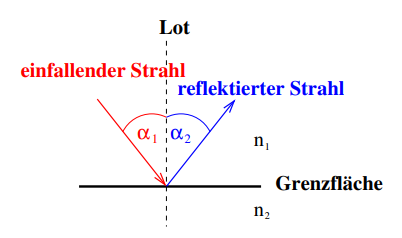
\includegraphics[height=3cm, keepaspectratio]{bilder/reflex.PNG}
        \caption{Reflexion.}\label{fig:reflex}
        \end{subfigure}%
        %
        \begin{subfigure}[b]{.33\linewidth}
        \centering
        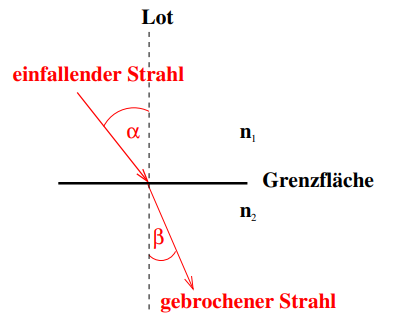
\includegraphics[height=3cm, keepaspectratio]{bilder/brech.PNG}
        \caption{Brechung.}\label{fig:brech}
        \end{subfigure}
        %
        \begin{subfigure}[b]{.33\linewidth}
        \centering
        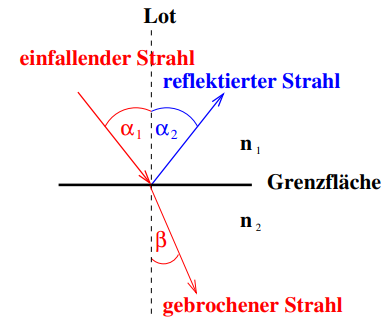
\includegraphics[height=3cm, keepaspectratio]{bilder/reflexUNDtrans.PNG}
        \caption{Reflexion und Transmission.}\label{fig:reflexUNDtrans}
        \end{subfigure}
        \caption{Systematische Darstellung der Brechung und Reflexion. \cite{anleitung}}
        \label{fig:alle_drei_bilder}
    \end{figure}


\subsection{Wellenoptik und Beugung}
\label{Beugung}
    Sobald Licht auf ein Hindernis trifft, das relativ klein zur eigenen Wellenlänge ist, breitet sich es im Schattenraum aus.
    Diese sogennante Beugung kann nicht mehr durch die Strahlenoptik erklärt werden, die Wellenoptik wird herangezogen.
    
    \subsubsection*{Wellenoptik}
        Für die elektromagnetische Welle ist die Frequenz $\nu$ bzw. Wellenlänge $\lambda$ sowie die Ausbreitungsgeschwindigkeit $v$ charakteristisch.
        Bei Überlagerung mehrerer Wellen addieren sich die Amplituden der Wellen in jedem Punkt.
        Nach dem Superpositionsprinzip folgt aus der Addition der Einzelintensitäten die resultierende Intensitätsverteilung.

        \noindent
        Weiterhin besteht Licht aus $\SI{1e-8}{\second}$ dauernden Wellenzügen.
        Bei gleicher Frequenz und fester Phasenbeziehung, kann ein Interferenzbild entstehen.
        Dabei wird zwischen konstruktive und destruktive Interferenz unterschieden.
        Beträgt der Gangunterschied genau $\sfrac{\lambda}{2}$, kommt es bei gleicher Intensität zur Auslöschung der Wellen.

    \subsubsection*{Beugung am Gitter}
        Mithilfe von Beugung am Gitter werden die daraus resultierenden Interferenzerscheinungen untersucht.
        Dabei kann die Ausbreitung einer Welle mithilfe des Huygenschen Prinzips definiert werden.
        %soll das prinzip noch erklärt werden?

        \noindent
        Die Beugung am Gitter kann zunächst vereinfacht werden, indem ein einfacher Spalt als Hindernis gesetzt wird.
        Nun trifft eine ebene Wellenfront auf diesen Spalt, alle Punkte in der Spaltöffnung werden dadurch gebeugt.
        Die resultierenden, gebeugten Wellen haben dabei dieselbe Frequenz und eine feste Phasenbeziehung.
        Hinter dem Spalt kann nun im Abstand $L$ ein Schirm gestellt werden, auf diesem ist dann das Interferenzmuster zu sehen, das aus dunklen und hellen Streifen besteht.
        Für die hellen Streifen besteht folgender Zusammenhang
        \begin{equation*}
            a \cdot \sin \alpha = k \cdot \lambda \, .
        \end{equation*}
        Die Spaltbreite wird mit $a$ beschrieben.
        Die Intensitätsminima können durchnummeriert werden, so befindet sich das $k$-te Intensitätsminimum in einem Winkel $\alpha$ relativ zur geradlinigen Ausbreitungsrichtung.

        \noindent
        Analog kann ein Ausdruck für ein Gitter aufgestellt werden.
        Bei einem Strichgitter mit $N$-Einfachspalten gleicher Breite und mit der Gitterkonstanten $d$, gilt bei senkrechtem Lichteinfall
        \begin{equation*}
            d \cdot \sin \alpha = k \cdot \lambda \, .
        \end{equation*}
        Hierbei ist $k$ der Index des zu betrachtenden Intensitätsmaximums.